% !TEX TS-program = pdflatex
% !TeX program = pdflatex
% !TEX encoding = UTF-8
% !TeX spellcheck = en_US

\documentclass[11pt, a4paper]{article}
%\usepackage{fullpage}
\usepackage[left=1cm,right=1cm,top=1cm,bottom=2cm]{geometry}
\usepackage[fleqn]{amsmath}
\usepackage{amssymb}
%\usepackage{indentfirst}
\usepackage[T1]{fontenc}
\usepackage[utf8]{inputenc}
\usepackage[french,english]{babel}
\usepackage{txfonts} 
\usepackage[]{graphicx}
\usepackage{multirow}
\usepackage{hyperref}
\usepackage{parskip}
\usepackage{multicol}
\usepackage{wrapfig}
\usepackage{multicol}

\usepackage{turnstile}%Induction symbole

\usepackage{tikz}
\usetikzlibrary{arrows, automata}
\usetikzlibrary{decorations.pathmorphing}

\renewcommand{\baselinestretch}{1}

\setlength{\parindent}{0pt}


\begin{document}
	
	%\pagestyle{empty} 
	\begin{tabular}{ll}
		\multirow{3}{*}{
\includegraphics[width=1.5cm]{../../extra/logo/esi.ml.pdf}} & \'Ecole national Supérieure d'Informatique, Algiers, Algeria\\
		& 2CSSID (2024/2025)\\
		& Machine Learning (ML)
	\end{tabular}\\[.25cm]
	\noindent\rule{\textwidth}{1pt}\\[-0.5cm]
	\begin{center}
		{\LARGE \textbf{Workshop 02: Data preparation and models' evaluation}}
		\begin{flushright}
			Mr. Abdelkrime ARIES
		\end{flushright}
	\end{center}\vspace{-.25cm}
	\noindent\rule{\textwidth}{1pt}
	
%	This workshop is about data preparation. 
%	Of course, we will not explore all methods; it is all about the chosen dataset.
%	Also, we will try to explore imbalanced data.
	
	\begin{center}
		\begin{tabular}{|p{.8\textwidth}|}
		\hline
		Apply some data preparation techniques \\
		Get familiar with CRISP-DM on a simple project\\
		Learn models' evaluation \\
		Try some tools: pandas, matplotlib, scikit-learn, imbalanced-learn \\
		\hline
	\end{tabular}
	\end{center}

\section*{Useful links}

\begin{itemize}
	\item \textbf{Dataset}: {\scriptsize \url{https://archive.ics.uci.edu/dataset/601/ai4i+2020+predictive+maintenance+dataset}} 
	\item \textbf{Demo}: {\scriptsize \url{https://github.com/projeduc/ESI_ML/blob/main/TP/SD_2022-2023/TP01/TP01_pretraitement_sujet.ipynb}}
	\item \textbf{MatplotLib}: {\scriptsize \url{https://matplotlib.org/stable/gallery/index.html}}
	\item \textbf{imbalanced-learn}: {\scriptsize \url{https://imbalanced-learn.org/stable/user_guide.html#user-guide}}
	\item \textbf{CRISP-DM (web)}: {\scriptsize \url{https://www.ibm.com/docs/en/spss-modeler/18.5.0?topic=dm-crisp-help-overview}}
	\item  \textbf{CRISP-DM (pdf)}: {\scriptsize \url{https://www.ibm.com/docs/en/SS3RA7_18.5.0/pdf/ModelerCRISPDM.pdf}}
\end{itemize}


\begin{multicols}{2}
	
\section{Business understanding}

The first step is to get a clear understanding of the business goals and needs for this project. 
Then, we will translate this knowledge into a well-defined data mining problem. 
Finally, we will create a preliminary plan outlining the steps needed to achieve those goals.

Predictive Maintenance is a proactive approach to equipment maintenance.
It uses data analytics and machine learning techniques to predict when machinery or systems are likely to fail. 
In our case, not only we want to detect if a machine is going to fail; but to detect one or more of these 5 failure modes:
tool wear failure (TWF), heat dissipation failure (HDF), power failure (PWF), overstrain failure (OSF) and random failures (RNF).
%\begin{itemize}
%	\item tool wear failure (TWF)
%	\item heat dissipation failure (HDF)
%	\item power failure (PWF)
%	\item overstrain failure (OSF)
%	\item random failures (RNF)
%\end{itemize}

To this end, we want to use all or part of these features:
\begin{itemize}
	\item product ID: consisting of a letter L, M, or H for low (50\% of all products), medium (30\%) and high (20\%) as product quality variants and a variant-specific serial number
	\item air temperature
	\item process temperature
	\item rotational speed: frequency of rotation of an object around an axis.
	\item torque: a measure of the force that can cause an object to rotate about an axis.
	\item tool wear: gradual failure of cutting tools due to regular operation
\end{itemize}

Discuss these solutions, given we want to use logistic regression:
\begin{enumerate}
	\item One model having the 5 outputs (TWF, HDF, PWF, OSF, RNF) with softmax function.
	\item One model having the 5 outputs (TWF, HDF, PWF, OSF, RNF, Other) with softmax function.
	\item One model having the 5 outputs (TWF, HDF, PWF, OSF, RNF) with sigmoid function.
	\item One model having the 5 outputs (TWF, HDF, PWF, OSF, RNF, Other) with sigmoid function.
	\item Two models, one for binary classification for failure yes/no. 
	In case of failure, we train a second model to detect the type similar to that of first solution.
	\item the same thing, but the second model is similar to that of the third solution. 
\end{enumerate}


\section{Data understanding}

In the data understanding phase, we first gather the available information. 
Then, we dive deep to get to know the data:  We check for quality issues, look for early clues about trends, and identify any intriguing patterns. 
This lets us form hunches about what the data might be hiding.

\subsection{Collecting initial data}

Let us suppose that data exists already. 
But, we have multiple sources: an sqlite3 database and a csv tabular.
\begin{itemize}
	\item Read the data using \textbf{pandas}:
	\begin{itemize}
%		\item Read the data using \textbf{pandas}. 
		\item Read \textbf{ai4i2020a.csv} which is a CSV file with comma as separation mark
		\item Read \textbf{ai4i2020b.sqlite} which has the following table
	\end{itemize} 
%	\item Read \textbf{ai4i2020a.csv} which is a CSV file with comma as separation mark
%	\item Read \textbf{ai4i2020b.sqlite} which has the following table
\end{itemize}

\begin{verbatim}
CREATE TABLE failure (
    ID VARCHAR(7) NOT NULL,
    Air_Temperature_K FLOAT,
    ProcessTemperature_K FLOAT,
    Rotational_speed INTEGER,
    Torque FLOAT,
    Tool_wear INTEGER,
    Failure INTEGER,
    TWF INTEGER,
    HDF INTEGER,
    PWF INTEGER,
    OSF INTEGER,
    RNF INTEGER
);
\end{verbatim}

\subsection{Describing data}

For each dataset, apply these techniques:
\begin{itemize}
	\item Show columns info using \textbf{pandas.DataFrame.info()}.
	\item If numerical values are not detected properly, fix it (check data types on the online dataset's description).
	\item Describe the dataset using \textbf{pandas.DataFrame.describe()}.
	\item Describe dataset 1 (CSV) when "\textit{Type}" == "L" (low).
	\item Show categories of non-unique categorical features.
\end{itemize}

\subsection{Exploring data}

For each dataset, apply these techniques:
\begin{itemize}
	\item Plot a pie chart for binary relation failure/not (Fig. \ref{res-explore}(a))
	\item Plot a pie chart for different failure classes (Fig. \ref{res-explore}(b))
	\item Draw the box plot of to temperature features for non null values (Fig. \ref{res-explore}(c)).
	\item If you detect any outliers, display them.
	\item Draw plot pie chart of "\textit{Type}".
	\item Apply PCA on "\textit{Air temperature}", "\textit{Process temperature}", "\textit{Rotational speed}", "\textit{Torque}" and "\textit{Tool wear}" to get a two dimensional representation. 
%	For simplicity, try the 500 first samples.
	\item Plot samples' distribution based on this representation so we can check classes' separability
\end{itemize}

\end{multicols}

\begin{figure}[ht]
	\centering
	\begin{tabular}{ccc}
		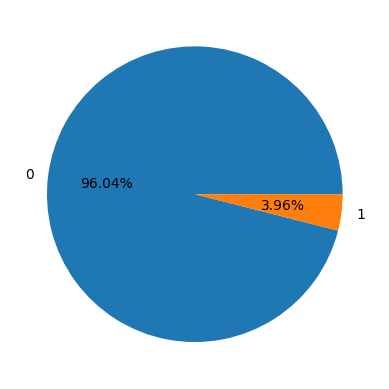
\includegraphics[width=0.22\textwidth]{bin_percentage.png} &
		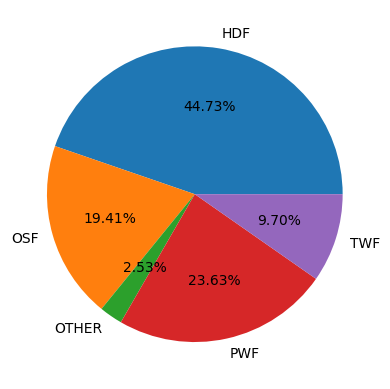
\includegraphics[width=0.22\textwidth]{failure_percentage.png} &
		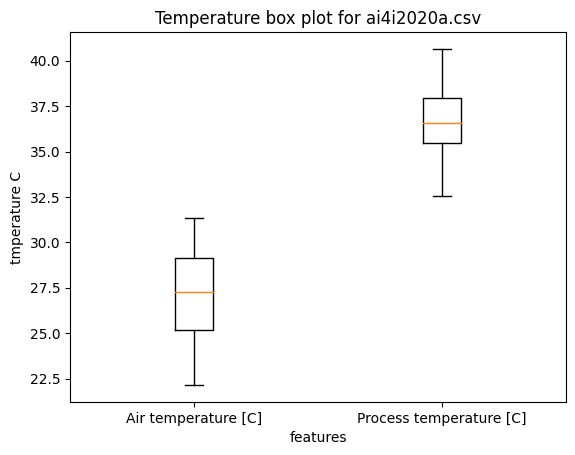
\includegraphics[width=0.22\textwidth]{box_plot.png} \\
		(a) Binary relations &
		(b) \% classes  &
		(c) Box plot \\
	\end{tabular}
	\caption{Exploring results}
	\label{res-explore}
\end{figure}

\begin{multicols}{2}
	
\subsection{Verifying data quality}

\begin{itemize}
	\item Show samples containing at least one omitted value
	\item Show samples which do not have a failure, but have a failure type (contradiction)
\end{itemize}

\section{Data preparation}

\subsection{Selecting data}

\begin{itemize}
	\item Do we need these features: "\textit{Product ID}" and "\textit{Machine failure}"? Why?
\end{itemize}

\subsection{Constructing new data}

\begin{itemize}
	\item Transform Celsius into Kelvin for temperature : $ K = C + 273.15 $
	\item Transform Failure types into one categorical column and delete original columns (dataset 1)
	\item Add another column for the failure type "OTHER" (dataset 2)
	\item If "\textit{Type}" does not exist, infer it from "\textit{Product ID}"
	\item Transform "\textit{Type}" into OneHot representation
\end{itemize}

\subsection{Integrating data}

\begin{itemize}
	\item Rename columns to get the same schema.
	\item Delete unshared columns (which exists only in one dataset).
	\item Merge the two tables into one.
\end{itemize}

\subsection{Cleaning data}

\begin{itemize}
	\item Delete all inconsistent samples (there is no failure yet there is a failure type)
	\item Find all duplicate samples using "\textit{product ID}"
	\item Replace all missing values from the same product (using "\textit{product ID}")
	\item Delete duplicates
	\item Delete "\textit{Product ID}" and "\textit{Failure}" (no need for those anymore)
	\item If a sample has more than a missing value, delete it
	\item Replace missing values by the average of the same type
\end{itemize}

\subsection{Formatting data and Constructing new data}

\begin{itemize}
	\item Put the classes at the end so we can select them easily.
	\item Split data into train (70\%) and test (30\%).
	\item Apply the oversampling \textbf{SMOTE} on training dataset to get a new one
	\item Apply two undersampling techniques on the majority class: \textbf{ClusterCentroids} and \textbf{TomekLinks} to get two new training datasets
	\item Apply normalization on the 4 past datasets to get three new ones
	\item In this case, we will have 8 training datasets: No\_sampling, No\_sampling\_normalized, SMOTE, SMOTE\_normalized, ClusterCentroids, ClusterCentroids\_normalized, TomekLinks and TomekLinks\_normalized.
	\item Separate inputs (X) and outputs (Y) for each of them
	\item Transform Y's into OneHot preserving the original one
\end{itemize}


\section{Modeling and Evaluation}

\begin{itemize}
	\item Train these models on the 8 datasets:
	\begin{itemize}
		\item Logistic regression with L2 penalization (by default) and "liblinear" solver.
		\item Gaussian Naïve Bayes 
		\item CART Decision tree
		\item Random forest with 50 estimators
	\end{itemize}
	\item For each of the 32 resulted models, get these information:
	\begin{itemize}
		\item Train time
		\item Test time
		\item Train accuracy
		\item Test accuracy
	\end{itemize}
	\item Show the table which summarizes these results
\end{itemize}

Let's discuss these results:
\begin{itemize}
	\item In terms of training time
	\begin{itemize}
		\item What is the order of the algorithms from fastest to slowest?
		\item Justify this based on how the algorithm constructs the model.
		\item How can we improve the training time of each algorithm (if we can)?
	\end{itemize}
	\item In terms of test time
	\begin{itemize}
		\item What is the order of the algorithms from fastest to slowest?
		\item Justify this based on how the model estimates the class.
		\item How can we improve the estimation time of each algorithm (if we can)?
	\end{itemize}
	\item In terms of training accuracy
	\begin{itemize}
		\item What is the order of the algorithms from best converged to worst?
		\item Justify this based on how the algorithm constructs the model.
	\end{itemize}
	\item In terms of test accuracy
	\begin{itemize}
		\item What is the order of the algorithms from best generalized to worst?
		\item Justify this based on how the model estimates the class.
	\end{itemize}
	\item In terms of used data
	\begin{itemize}
		\item How normalization has affected the results?
		\item How sampling (over-sampling and under-sampling) has affected the results?
	\end{itemize}
\end{itemize}

\end{multicols}


\end{document}
